% An Overview of Lie Algebra's
% Adapted from Justin Ryan's "Examples of Lie Algebras"
% Chaskin Saroff and Alexander Jansing	
% last changed: 3 May 2015
% feel free to make any improvements/changes you wish

\documentclass[9 pt]{beamer}
\usepackage{etex}
\reserveinserts{36}
% \usepackage{default}
\usepackage{lmodern}
\usepackage{amsmath,amsfonts,epsfig,pgf} % ,graphicx
\usepackage{graphicx}
\usepackage{hyperref}

% choose your theme
 \usetheme{Warsaw} % Warsaw, Copenhagen, Darmstadt, Madrid, Singapore, etc...

% custom SUNY Polytechnic color scheme
\definecolor{polytechnic}{rgb}{0.05,0.1,0.7}
\setbeamercolor*{palette primary}{fg=white, bg=polytechnic}
\setbeamercolor*{palette sidebar primary}{fg=black, bg=polytechnic}
\setbeamercolor{block title}{bg=black,fg=white} % bg=background, fg= foreground
\setbeamercolor{block body}{bg=polytechnic,fg=black} % bg=background, fg= foreground
\setbeamercolor{alerted text}{fg=polytechnic}
\usecolortheme[named={polytechnic}]{structure}
\def\today{\number\day\space\ifcase\month\or
   January\or February\or March\or April\or May\or June\or
   July\or August\or September\or October\or November\or December\fi
   \space\number\year}

% something I found to get alert blocks in the polytechnic color scheme
\newenvironment<>{lakeblock}[1]{%
  \begin{actionenv}#2%
      \def\insertblocktitle{#1}%
      \par%
      \mode<presentation>{%
\setbeamercolor{block title}{fg=white,bg=black}
       \setbeamercolor{block body}{fg=white,bg=polytechnic}
            }%
      \usebeamertemplate{block begin}}
    {\par\usebeamertemplate{block end}\end{actionenv}}

% polytechnic State logo on every page
%\logo{\pgfputat{\pgfxy(-10.5,0.35)}{\pgfbox[center,center]
%{\includegraphics[height=1.35cm]{polytechnic_logo_horiz_grn}}}}

% commutative diagrams with XY-pic
\usepackage[all]{xy}
\SelectTips{cm}{}
% make \mathscr, TeX \cal, and Euler script *all* available
% (notice the new command names to avoid overlap and/or confusion)
\usepackage{mathrsfs}
\let\rscr=\mathscr % use \rscr{} for Ralph Smith fancy script
\let\mathscr=\relax
\let\mcal=\mathcal % use \mcal{} for TeX \cal script
\usepackage{eucal}
\let\escr=\mathcal % use \escr{} for Euler script
\let\mathcal=\relax
% a better "bar" thanks to Donald Arsenau -- see \pbar infra
\usepackage{accents}

% title page information
\title[The Deutsch-Jozsa problem: de-quantisation and entanglement]{The Deutsch-Jozsa problem: de-quantisation and entanglement}
\author[A. Abbott]{Alastair A. Abbott}
\institute[University of Auckland]{
\includegraphics[height = 2cm]{auckland}}
\date{\today}

% new math commands
\newcommand{\at}[1]{\emph{\alert{#1}}}
\newcommand{\ad}[1]{\text{ad}_{#1}}
\newcommand{\add}[1]{\ad{#1}^\dagger}
\newcommand{\br}[2]{\left[ #1, #2 \right]}
\newcommand{\bre}{\br{\ }{\,}}
\newcommand{\C}{\mathbb{C}}
\newcommand{\F}{\mathbb{F}}
\newcommand{\h}{\lag{h}}
\newcommand{\inp}[2]{\langle #1, #2 \rangle}
\newcommand{\inpe}{\inp{\ }{\,}}
\newcommand{\lag}[1]{\mfrak{#1}}
\newcommand{\mfrak}[1]{\mathfrak{#1}}
\newcommand{\R}{\mathbb{R}}
\renewcommand{\a}{\alpha}
\newcommand{\surj}{\rightarrow\kern-.82em\rightarrow}
\newcommand{\tQ}{\widetilde{Q}}
\renewcommand{\v}{\lal{v}}
\newcommand{\z}{\lal{z}}
\newcommand{\V}{\mathfrak{g}}
\newcommand{\fg}{\mathfrak{g}}
\newcommand{\ff}{\mathfrak{f}}
\newcommand{\fz}{\mathfrak{z}}
\newcommand{\fv}{\mathfrak{v}}
\newcommand{\fh}{\mathfrak{h}}
\newcommand{\QQ}{\mathbb{Q}}
\newcommand{\ZZ}{\mathbb{Z}}
\newcommand{\RR}{\mathbb{R}}
\newcommand{\CC}{\mathbb{C}}
\newcommand{\NN}{\mathbb{N}}
\newcommand{\FF}{\mathbb{F}}
\newcommand{\zvec}{\mathbf{0}}
\newcommand{\lal}[1]{\mathfrak{#1}}
\newcommand{\lan}{\lal{n}}
\newcommand{\lav}{\lal{v}}
\newcommand{\laz}{\lal{z}}
%\renewcommand{\span}[1]{\text{span}\left\{#1\right\}}
\def\ket#1{\big|{#1}\big>}
\def\bra#1{\big<{#1}\big|}
\def\braket#1#2{\big<{#1}\big|{#2}\big>}
\def\ketbra#1{\big|{#1}\big>\big<{#1}\big|}

% colored text commands
\newcommand{\red}[1]{{\color{red} #1}}
\newcommand{\grn}[1]{{\color{green} #1}}
\newcommand{\blu}[1]{{\color{blue} #1}}
\newcommand{\ylw}[1]{{\color{yellow} #1}}
\newcommand{\mgn}[1]{{\color{magenta} #1}}
\newcommand{\cyn}[1]{{\color{cyan} #1}}

%Stuff from Justin's example
%\renewcommand{\a}{\vect{a}}
%\newcommand{\abs}[1]{\vert #1 \vert}
%\renewcommand{\b}{\vect{b}}
%\newcommand{\bve}{\pbar{\ve}}
%\newcommand{\dps}{\displaystyle}
%\newcommand{\ds}{\oplus}
%\newcommand{\name}{{\bf Name:}\underline{\hspace{3 in}}}
%\newcommand{\nin}{\noindent}
%\newcommand{\norm}[1]{\left\Vert #1 \right\Vert}
%\newcommand{\pg}[1]{\paragraph{#1}}
%\newcommand{\ph}[1]{\phantom{#1}}
%\renewcommand{\span}[1]{\textrm{span}\left\{ #1 \right\}}
\renewcommand{\t}{\texttt{t}}
\newcommand{\T}{\textsc{T}}
\renewcommand{\u}{\vect{u}}
\renewcommand{\v}{\vect{v}}
\newcommand{\ve}{\varepsilon}
\newcommand{\vc}[1]{\left\langle #1 \right\rangle}
\newcommand{\vect}[1]{\mathbf{#1}}

% tiks packages
\usepackage{tikz}
\usetikzlibrary{calc}
\usepackage{tikzscale}
\usepackage{filecontents}
\usepackage{caption}
\usepackage{subcaption}
\captionsetup{compatibility=false}
\usepackage{wrapfig}

\newcommand{\tikzmark}[1]{\tikz[overlay,remember picture] \node (#1) {};}
\newcommand{\DrawBox}[1][]{%
    \tikz[overlay,remember picture]{
    \draw[red,#1]
      ($(left)+(-0.2em,0.9em)$) rectangle
      ($(right)+(0.2em,-0.3em)$);}
}


%%%ENUMERATE OVER SLIDES%%%
\newcounter{sauvegardeenumi}
\newcommand{\asuivre}{\setcounter{sauvegardeenumi}{\theenumi}}
\newcommand{\suite}{\setcounter{enumi}{\thesauvegardeenumi}}
%%%%%%%%%%%%%%%%%%%%%%%%%%%

\NewDocumentCommand{\highlight}{O{blue!40} m m}{%
    \draw[mycolor=#1] (#2.north west)rectangle (#3.south east);
}

\NewDocumentCommand{\fhighlight}{O{blue!40} m m}{%
    \draw[myfillcolor=#1] (#2.north west)rectangle (#3.south east);
}

\begin{document}

\begin{frame}{}

\titlepage

Alexander Jansing, Brittany Zeo  \\

\includegraphics[height=1cm]{suny_poly}\\


\end{frame}
\section{Definition}
\begin{frame}{Definitions}
What is \emph{de-quantisation}?
\begin{enumerate}
\item[] De-quantisation is taking a \emph{quantum algorithm} and computing its \emph{classical algorithm} counterpart.\pause
\item[] Classical algorithms are algorithms that can be computed on a Turing machine.
\item[] Quantum algorithms are algorithms that can be computed by a sequence of unitary operators.\pause
\item[] The \emph{oracle computational problem} means that an input is given and we use a black-box and the goal is to find something out about the black-box.
\end{enumerate}
\end{frame}

\section{Deutsch's problem}

\begin{frame}{Deutsch's problem} 
Deutsch's problem considers a Boolean function 
$$\mathfrak{f}: \{0,1 \} \rightarrow \{0,1 \},$$
and we're given an oracle to compute $\mathfrak{f}$. Deutsch's problem is to determine whether or not $\mathfrak{f}$ is balanced or constant in as few calls as possible.
\end{frame}

\subsection{Quantum Solution}
\begin{frame}{Quantum Solution}
Using only call to the quantum black-box computing $\mathfrak{f}$, we can determine with probability $1$ if $\mathfrak{f}$ is balanced or constant.

The quantum black-box can be described as the unitary operator 
$$U_\mathfrak{f}\ket{x}\ket{y} = \ket{x}\ket{y \oplus \mathfrak{f}(x)}.$$\pause
Noting that\\
$\begin{array}{ccccc}
U_\mathfrak{f}(U_\mathfrak{f}\ket{x}\ket{y}) &=& U_\mathfrak{f}\ket{x}\ket{y \oplus \mathfrak{f}(x)} &=& \ket{x}\ket{y \oplus \mathfrak{f}(x) \oplus \mathfrak{f}(x)}\\
&=&\ket{x}\ket{y},&
\end{array}$\\\pause
shows that\\
$$U_\mathfrak{f}U_\mathfrak{f} = \mathbb{I} \cdots$$\pause
Measuring the first qubit we obtain with probability $1$
\begin{enumerate}
\item[$\cdot$] $0$ if $\ff$ is constant,
\item[$\cdot$] and $1$ if $\ff$ is balanced.
\end{enumerate}
\end{frame}

\subsection{Classical Solutions}
\begin{frame}{Classical Solution}
In the classical solution, we can use the set $\{1, i\}$ as a computational basis just as the quantum calculations use $\{\ket{0}, \ket{1} \}$.\\
\vspace*{.5cm}
Now an arbitrary $z = a + bi $, where $z \in \CC$ and $a,b\in\RR$, has a natural superposition of the basis elements. And we can think of a classical black-box, 
\begin{center}
$C_\ff : \CC \rightarrow \CC$, that is analogous to the quantum $U_\ff : \{0,1 \} \rightarrow \{0,1 \}$.\pause
\end{center}
\begin{enumerate}
\item[$\cdot$] If $\ff$ is constant, $C_\ff$ is the identity operation to within a factor of $-1$.
\item[$\cdot$] If $\ff$ is balanced, $C_\ff$ is the conjugate operation. \pause
\end{enumerate}
In order to observe our results, we need to be able to project these complex numbers to the computational basis. Which can be done by multiplying the input so that the output is purely imaginary or real.
\end{frame}

\section{Deutsch-Jozsa problem}
\begin{frame}{Deutsch-Jozsa problem}
The Deutsch-Jozsa problem is an expansion on the original Deutsch problem that works on a general case of $n$-bit inputs.\\
So $\ff: \{0,1\}^n \rightarrow \{0,1\}$ and suppose we are given a black-box computing $\ff$ with the guarantee that $\ff$ is constant or balanced.\pause \\ \vspace*{.3cm}
Like the Deutsch problem, the Deutsch-Jozsa problem tried to determine if $\ff$ is constant or balanced in as few calls as possible. Unlike Deutsch's problem, the distribution of constant and balanced is asymmetrical in the Deutsch-Jozsa problem.\\ \vfill
In general, there are $N = 2^n$ possible input stings, each with two possible outputs (0 or 1). Hence for any $n$, there are $2^N$ ($2^{2^n}$) possible functions, $\ff$.\pause \\
Of these, exactly two are constant and $\left( \begin{array}{c}
									N\\ N/2									
									\end{array} \right)$ are balanced.
\end{frame}

\section{Adaptation for $n = 2$}
\subsection{Quantum Solution}
\begin{frame}{Quantum Solution}
For $n = 2$ the quantum black-box is given three qubits. We initially prepare our system in the state $\ket{00}\ket{1}$, and apply $H^{\otimes 3}$... \pause\\
\vspace*{.2cm} This state is separable iff $(-1)^{\ff(00)}(-1)^{\ff(11)}c_{00}c_{11} = (-1)^{\ff(01)}(-1)^{\ff(10)}c_{01}c_{10}$.\\
The state is further simplified by nothing that the mapping $$(-1)^{\ff(a)}(-1)^{\ff(b)} \iff \ff(a) \oplus \ff(b); a,b \in \{0,1\}^2$$ is a bijection.\\ \pause
\vspace*{.2cm} And the separability condition reduces to $\ff(00) \oplus \ff(11) = \ff(01) \oplus \ff(10)\cdots$ \\\pause
By measuring both qubits if both are measured as $0$ then $\ff$ is constant, otherwise $\ff$ is balanced.
\begin{center}
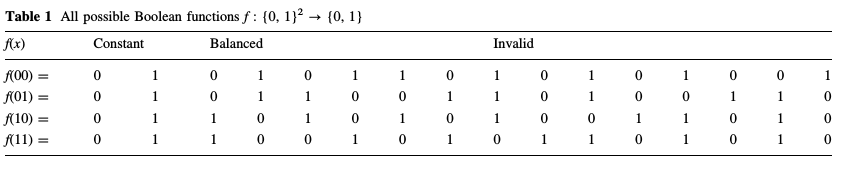
\includegraphics[height = 1.9cm]{table1}
\end{center}
\end{frame}

\subsection{Classical Solution}
\begin{frame}{Classical Solution}
We can extend the classical $C_\ff : \CC \rightarrow \CC$ to two inputs and it becomes $$C_\ff : \CC^2 \rightarrow \CC^2.$$
Let $z_1, z_2$ be complex numbers, \begin{center}
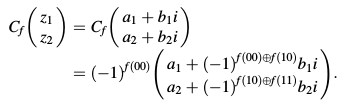
\includegraphics[height = 2cm]{eq4}
\end{center}
\end{frame}

\begin{frame}{Classical Solution}
\begin{center}
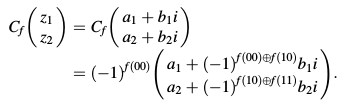
\includegraphics[height = 1.3cm]{eq4}
\end{center}
To project each qubit back onto the computation basis, we multiply each of the complex numbers that the black-box output by their respective inputs.\pause \\
Let $z_1 = z_2 = 1 + i$, and we get the following:
\begin{center}
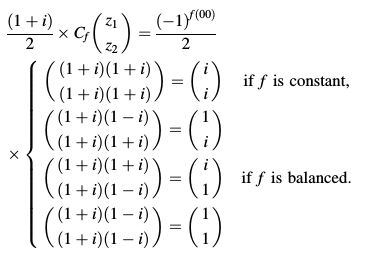
\includegraphics[height = 3.6cm]{eq5}
\end{center}
\end{frame}

\begin{frame}{Classical Solution}
Let $z_1 = z_2 = 1 + i$, and we get the following:
\begin{center}
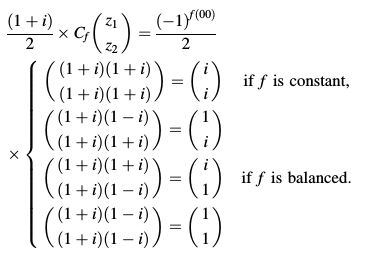
\includegraphics[height = 3.6cm]{eq5}
\end{center}
If both complex numbers are imaginary, then $\ff$ is constant; otherwise it is balanced.
\end{frame}

\section{Conclusion}
\begin{frame}{Conclusion}
Because the quantum solution is separable, it is possible to write the output as a list of two complex numbers, otherwise finding a classical solution in this fashion would have required a list of complex numbers exponential in the number of input qubits.\\
\vfill Due to time constraints, proofs are omitted.
\end{frame}
\end{document}











































